\documentclass[a4paper,11pt,leqno]{report}\usepackage[]{graphicx}\usepackage[]{color}
%% maxwidth is the original width if it is less than linewidth
%% otherwise use linewidth (to make sure the graphics do not exceed the margin)
\makeatletter
\def\maxwidth{ %
  \ifdim\Gin@nat@width>\linewidth
    \linewidth
  \else
    \Gin@nat@width
  \fi
}
\makeatother

\definecolor{fgcolor}{rgb}{0.345, 0.345, 0.345}
\newcommand{\hlnum}[1]{\textcolor[rgb]{0.686,0.059,0.569}{#1}}%
\newcommand{\hlstr}[1]{\textcolor[rgb]{0.192,0.494,0.8}{#1}}%
\newcommand{\hlcom}[1]{\textcolor[rgb]{0.678,0.584,0.686}{\textit{#1}}}%
\newcommand{\hlopt}[1]{\textcolor[rgb]{0,0,0}{#1}}%
\newcommand{\hlstd}[1]{\textcolor[rgb]{0.345,0.345,0.345}{#1}}%
\newcommand{\hlkwa}[1]{\textcolor[rgb]{0.161,0.373,0.58}{\textbf{#1}}}%
\newcommand{\hlkwb}[1]{\textcolor[rgb]{0.69,0.353,0.396}{#1}}%
\newcommand{\hlkwc}[1]{\textcolor[rgb]{0.333,0.667,0.333}{#1}}%
\newcommand{\hlkwd}[1]{\textcolor[rgb]{0.737,0.353,0.396}{\textbf{#1}}}%
\let\hlipl\hlkwb

\usepackage{framed}
\makeatletter
\newenvironment{kframe}{%
 \def\at@end@of@kframe{}%
 \ifinner\ifhmode%
  \def\at@end@of@kframe{\end{minipage}}%
  \begin{minipage}{\columnwidth}%
 \fi\fi%
 \def\FrameCommand##1{\hskip\@totalleftmargin \hskip-\fboxsep
 \colorbox{shadecolor}{##1}\hskip-\fboxsep
     % There is no \\@totalrightmargin, so:
     \hskip-\linewidth \hskip-\@totalleftmargin \hskip\columnwidth}%
 \MakeFramed {\advance\hsize-\width
   \@totalleftmargin\z@ \linewidth\hsize
   \@setminipage}}%
 {\par\unskip\endMakeFramed%
 \at@end@of@kframe}
\makeatother

\definecolor{shadecolor}{rgb}{.97, .97, .97}
\definecolor{messagecolor}{rgb}{0, 0, 0}
\definecolor{warningcolor}{rgb}{1, 0, 1}
\definecolor{errorcolor}{rgb}{1, 0, 0}
\newenvironment{knitrout}{}{} % an empty environment to be redefined in TeX

\usepackage{alltt}

\usepackage{amsmath, amssymb, mdframed, caption, subcaption, graphicx, enumitem}
\usepackage{nicefrac}

\usepackage{hyperref}
\hypersetup{colorlinks=true, urlcolor=blue, breaklinks=true}

\newmdtheoremenv{Definition}{Definition}[chapter]
\newmdtheoremenv{Exercise}[Definition]{Exercise}
\newmdtheoremenv{Theorem}[Definition]{Theorem}
\newmdtheoremenv{Lemma}[Definition]{Lemma}

\newcommand{\supp}{\operatorname{supp}} 
\newcommand{\E}{\mathbb{E}}
\newcommand{\eps}{\varepsilon}

\newcommand{\N}[2]{\mathcal{N}\left( #1, #2 \right)}	

\newcommand{\philip}[1]{ \textcolor{red}{\textbf{Philip:} #1}}
\newcommand{\chris}[1]{ \textcolor{blue}{\textbf{Chris:} #1}}

\title{Basic Probability}
\date{}

%% Load R packages


\IfFileExists{upquote.sty}{\usepackage{upquote}}{}
\begin{document}

\setcounter{chapter}{5}


\chapter{The Gaussian Distribution}

If there is any one distribution that has traversed mathematics and found a home in cultural memory, it surely is the \textbf{Gaussian} or \textbf{normal distribution}
(both names are common and we will use them interchangeably here). 
Not only is it super-useful in many data modelling applications, it also has a host of convenient mathematical properties, some of which we are going
to explore in this chapter. 

Before going into any detail, let us first motivate this distribution. What we want is a distribution on a real vector space ($ \mathbb{R}^{n} $). We will
start out with the simplest case and fist look at the Gaussian distribution on the real line. Our desiderata for the Gaussian\footnote{Notice that Gauss' original
motivation was different from ours. While we are giving a largely geometric account of the normal distribution, Gauss was concerned with finding a distribution
on $ n $ independent points whose maximum likelihood estimate (See Section~\ref{eq:parameterEstimation}) would be the mean of those points.} are as follows:
\begin{itemize}
\item The distribution should be centred around one specific point which we will call the mean.
\item The more distant a point is from the mean, the less probable it should be.
\item The distance metric should be adjustable so as to assign distant points more or less probability as needed.
\item Equally distant points should have the same probability, independent of their direction.
\end{itemize}

\section{The Univariate Gaussian}

The Gaussian distribution is one of the most important and most widely used distributions in all of statistics. The reason is that many natural observations
tend to be normally distributed. Many other distributions are also based on it or can be approximated by a Gaussian. Finally, there are several mathematical
properties of the Gaussian that make calculating with it rather easy. In this section we will look at the \textbf{univariate} Gaussian distribution, that is
the Gaussian distribution in one dimension. In Section~\ref{sec:mvGauss} we will also see how to model data in $ \mathbb{R}^{n} $ that is extremely complexly 
structured with \textbf{multivariate} Gaussian distributions.

\begin{figure}
\center
\begin{knitrout}
\definecolor{shadecolor}{rgb}{0.969, 0.969, 0.969}\color{fgcolor}
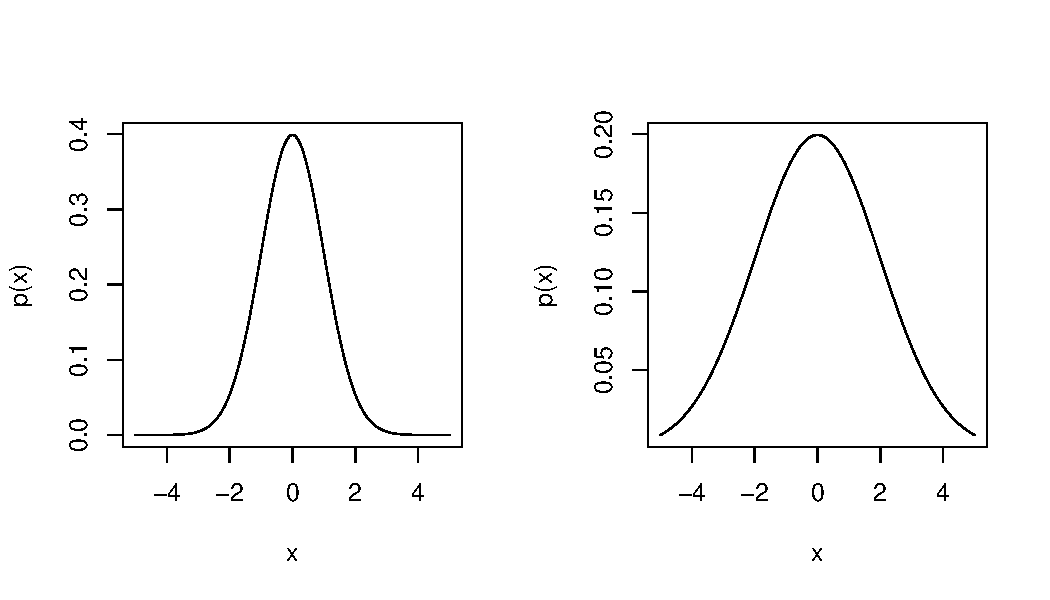
\includegraphics[width=\maxwidth]{figures/uniGauss-1} 

\end{knitrout}
\caption{Standard normal density (left) and with variance $ \sigma^{2} = 2 $ (right).}
\label{fig:uniGauss}
\end{figure}

\subsection{Deriving the density}

What we want is a distribution that models spatial data, i.e.\ data that lives in some vector space. There should be a centre of mass around which the data concentrates
and deviation from that centre of mass should be ``penalized'', meaning that the further away from the centre a data point is, the less probable it should be.
Since we are interested in modelling spatial data in real vector spaces, we will choose the \href{https://en.wikipedia.org/wiki/Euclidean_distance}{Euclidian
distance} as a distance measure. In the case of one dimension, the Euclidean distance is simply the absolute difference. For $ x,y \in \mathbb{R} $, the Euclidian
distance is $ (y - x)^{2} $. Notice that this is symmetric as any good distance metric should be. 

As it looks right now, all deviations are going to be penalized to the same extent. In other words: the Euclidian distance is linear in the difference of two points.
What if we want to be a bit stricter and penalize points that are far away from the centre even more or conversely, if we wanted to be lenient and diminish the penalty
for deviation from the centre? In such a case we would have to scale the Euclidian distance. In fact, there is a generalization of the Euclidean distance that
allows for scaling. It is called the \href{https://en.wikipedia.org/wiki/Mahalanobis_distance}{Mahalanobis distance}. In the one-dimensional case, it introduces
a scale factor by which the difference between two points is scaled. The Mahalanobis distance between $ x,y \in \mathbb{R} $ is 
\begin{equation*}
\left(\frac{x - y}{\sigma}\right)^{2} \, ,
\end{equation*}
where $ \sigma > 0 $ is an adjustable scale factor. If $ \sigma < 1 $ it will exaggerate the difference between $ x $ and $ y $ and hence lead to a greater
penalty for distant points. Conversely, if $ \sigma > 1 $ it will lessen the difference between $ x $ and $ y $ and therefore lead to a smaller penalty for 
distant points. The square of $ \sigma $ is called the \textbf{variance} and used to parametrize the Gaussian distribution, while $ \sigma $ itself is 
known as the \textbf{standard deviation}.

Now that we have found an appropriate (and adjustable!) distance metric, we have to turn it into a probability density. The standard way of turning any quantity
into a probability density is by simply exponentiating it. This way, it is guaranteed to be positive. In the present case, we actually want that the probability
decreases as the distance between the two points increases. Thus we are actually going to exponentiate the negative of the Mahalanobis distance. Finally, we
might want to differentiate that distance at some point. Whenever we do so we are going to have to deal with the squaring function. In order to make our lives
easier when differentiating, we also prefix the Mahalanobis distance with $ \nicefrac{1}{2} $ before exponentiating it. The result is
\begin{equation}
\exp\left(-\frac{1}{2} \left(\frac{x - y}{\sigma}\right)^{2} \right) \ .
\end{equation}

Notice that so far we have one adjustable parameter in that expression, namely the scale factor $ \sigma $ from the Mahalanobis distance. Initially we said
that points which follow a Gaussian distribution should be arranged around a centre which is more commonly known as the \textbf{mean}. 
Let us call this mean $ \mu $. In order to vary the location of the centre,
we turn $ \mu $ into a parameter (we simply replace $ y $ with $ \mu $). To recap, $ \mu $ determines the location
of the centre of the Gaussian density and $ \sigma $ scales it. The parameters are therefore called \textbf{location parameter} and \textbf{scale parameter}, respectively.
We now have an expression that is proportional to the Gaussian density. Whenever a RV $ X $ is distributed according to a normal distribution with location parameter
$ \mu $ and scale parameter $ \sigma $, we write $ X \sim \N{\mu}{\sigma} $. The corresponding density is
\begin{equation}
p(x) \propto \exp\left(-\frac{1}{2} \left(\frac{x - \mu}{\sigma}\right)^{2} \right) \ .
\end{equation}
In order to get a proper density, we still need to normalize. This requires a non-trivial integration that falls without the scope of this subsection\footnote{If
you are interested in seeing several different proofs, check \href{https://en.wikipedia.org/wiki/Gaussian_integral}{this wikipedia entry}. Laplace's proof is probably the easiest to follow.}. We
will just state the normalizing factor here. The full univariate normal density with parameters $ \mu $ (mean) and $ \sigma^{2} $ (variance) is
\begin{equation}
p(x) = \frac{1}{\sqrt{2\pi}\sigma} \exp\left(-\frac{1}{2} \left(\frac{x - \mu}{\sigma}\right)^{2} \right) \ .
\end{equation}

Notice that we do actually never \chris{better: rarely?} need this general density. Why? We can transform any Gaussian distribution into a \textbf{standard normal distribution}. This is 
the normal distribution with 0 mean and unit variance $ \N{0}{1} $. It is so important that it even has its own notation. 
\begin{equation}
\Phi(x) := p(x) \mbox{ where } X \sim \N{0}{1}
\end{equation}

\begin{Exercise}
Order the points $ 0.5 $, $ 0.8 $ and $ 1 $ according to their probability under $ \N{0.7}{10} $.
\end{Exercise}

%Any Gaussian variable can be normalized to a standard normal variable. This is often done in many applications.
%
%\begin{Exercise}
%Show that for $ X \sim \N{\mu}{\sigma^{2}} $ we have $ \frac{X - \mu}{\sigma} \sim \N{0}{1} $. The processes of subtracting the mean and dividing
%by the standard deviation are called centering and normalization, respectively. If both are performed we say that we standardise the RV.
%\end{Exercise}

\section{The Multivariate Gaussian$ ^{*} $}\label{sec:mvGauss}

Our goal in this section is to define a Gaussian distribution on $ \mathbb{R}^{n} $. This will require quite a bit of linear algebra. Readers who have not taken
a linear algebra course are advised to skip this section.

Let us start out by considering a random vector whose $ n $ dimensions are independent. That means that the probability of the vector can be factorised.
\begin{equation}
p(\vec{x}) = \prod_{i=1}^{n} p(x_{i})
\end{equation}
If each of the dimensions is distributed according to the same Gaussian $ \mathcal{N}(\mu, \sigma^{2}) $, we can easily generate random vectors of this form by taking $ n $ independent samples from the Gaussian.

Unfortunately, this severely limits our ability to model data. Not only can we never model correlations between dimensions, we also require that all dimensions
have the same variance. The data that we can model needs to be extremely homogeneous.

We could lessen this problem by drawing each random dimension from a different Gaussian. In this way, we would be able to assign different means and variances to different
dimensions. However, we could still not capture covariances\chris{what is this? readers don't know at this point, or do they? maybe give some quick recall}. What we need is a single Gaussian over $ \mathbb{R}^{n} $ which will allow us to model (potentially) dependent
dimensions. Having a mean vector with different mean values per dimension is trivial. In fact, we will further \chris{what do you mean by ``further'', it sounds like ``additionally'' and then it does not make sense} assume that the means of the dimensions are independent of
each other. Thus our mean vector will simply be 
$ \vec{\mu} = \begin{bmatrix}
\mu_{1} & \ldots & \mu_{n}
\end{bmatrix} $. We only demand that the variances of the dimensions may be correlated. To express such correlations we need to compactly store the variances and 
covariances of the dimensions. To do this, we introduce \textbf{covariance matrices}.

\subsection{Covariance Matrices}

\begin{Definition}[Covariance matrix]
A $ n \times n $ matrix $ \Sigma $ is called a covariance matrix of an $ n $-dimensional RV $ X $ if for $ 0 < i,j \leq n $ 
$$ \Sigma_{j,i} = cov(X_{j}, X_{i}) \ . $$ \chris{why flipping the indices?}
\end{Definition}

The covariance matrix has a couple of important properties which we will use when computing with it.
\begin{enumerate}
\item \textbf{Symmetry:} follows from the definition and the symmetry of the covariance.
\item \textbf{positive semi-definiteness:} See below.
\end{enumerate}
Notice that some authors will actually define covariance matrices to be symmetric, positive semi-definite matrices. This is fine in so far as any matrix with
these properties is a valid covariance matrix. When we construct models of data, we may actually simply stipulate the (co)-variances and thus build a covariance matrix.

\textbf{Proof of positive semi-definiteness} Recall that a $ n \times n $ matrix $ M $ is positive semi-definite (PSD) 
if for all $ \vec{z} \in \mathbb{R}^{n}\setminus \{0\} $ it holds
that $ \vec{z}^{\top}M\vec{z} \geq 0 $. Observe that we can write a covariance matrix $ \Sigma $ as the expectation of an outer product. 
\begin{equation}
\Sigma = \E\left[(\vec{X} - E[\vec{X}])^{\top}(\vec{X} - E[\vec{X}])\right]
\end{equation}
For all $ \vec{z} \in 
\mathbb{R}^{n}\setminus \{0\} $ we have
\begin{align}
\vec{z}\Sigma \vec{z}^{\top} 
&= \vec{z} \E\left[(\vec{X} - E[\vec{X}])^{\top}(\vec{X} - E[\vec{X}])\right] \vec{z}^{\top} \\
&=  \E\left[ \vec{z} (\vec{X} - E[\vec{X}])^{\top}(\vec{X} - E[\vec{X}]) \vec{z}^{\top} \right] \\
&= \E\left[(\vec{X} - E[\vec{X}])\vec{z}^{\top}\vec{z} (\vec{X} - E[\vec{X}])^{\top} \right] \\
&= \E\left[(\vec{X} - E[\vec{X}])c (\vec{X} - E[\vec{X}])^{\top} \right] \\
&= c \E\left[(\vec{X} - E[\vec{X}]) (\vec{X} - E[\vec{X}])^{\top} \right] \geq 0
\end{align}
where $ c $ is some positive constant. The result essentially follows from the linearity of expectation. 

The importance of being positive semi-definite may not be immediately apparent. It lies in the fact that many results are easily proven for positive semi-definite 
matrices. Any result that holds for positive semi-definite matrices also holds for covariance matrices. We will occasionally use this property in our proofs below.

Another important result is based solely on the symmetry of the matrix. By the spectral theorem we know that any symmetric matrix $ M $ can be factorized as
\begin{equation}\label{eq:eigenvalueDecomp}
M = U \Lambda U^{-1}
\end{equation}
where $ \Lambda $ is a diagonal matrix and $ U $ is orthonormal. Let us try to interpret this decomposition. The orthonormal matrix $ U^{-1} $ is a linear map from
$ \mathbb{R}^{n} $ to $ \mathbb{R}^{n} $. It effectively rotates the input. The matrix $ \Lambda $ then scales each row of the input and finally the matrix
$ U $ rotates the scaled input back. From the spectral theorem we know that the entries of $ \Lambda $ are the eigenvalues of $ M $. Therefore, the columns of $ U $
are the corresponding eigenvectors normalized to unit length. The decomposition thus gives us an efficient \chris{what do you mean by ``efficient''???} way of finding the eigenvalues of $ M $. We are now going
to show that these eigenvalues are always non-negative for PSD matrices.

\begin{Lemma}[Positive Eigenvalues]
Eigenvalues of PSD matrices are non-negative.
\end{Lemma}
\paragraph{Proof}  Assume this was not the case. Let $ z $ be an eigenvector of a positive 
semi-definite matrix $ A $ with negative eigenvalue $ \lambda < 0$. Then we get $ z^{\top}Az = z^{\top}\lambda z = \lambda z^{\top} z < 0 $ which contradicts the
premise that $ A $ is positive semi-definite. $ \square $

The lemma in turn implies that PSD matrices always have roots. These roots can easily be defined as $M^{\nicefrac{1}{2}} := U \Lambda^{\nicefrac{1}{2}} U^{-1}$ because
\begin{equation}\label{eq:PSDRoots}
(M^{\nicefrac{1}{2}})^2 = U \Lambda^{\nicefrac{1}{2}}U^{-1} U \Lambda^{\nicefrac{1}{2}} U^{-1}  =  U\Lambda^{\nicefrac{1}{2}}\Lambda^{\nicefrac{1}{2}} U^{-1} = M\ .
\end{equation} 

Covariance matrices are not always used in practice. It is sometimes more convenient to use their inverse instead. That inverse, $ \Sigma^{-1} $, is called a \emph{precision
matrix}. The names are telling: The entries in the covariance matrix measure to what extend two dimensions grow or shrink in relation to each other. The higher
that value the more deviation from the mean we will observe. 
The entries in the precision matrix tell us how precise (i.e.\ how close to the mean) the distribution is. Higher
precisions mean that we are going to observe less deviation from the mean vector.

\subsection{Deriving the density}

Now that we have learned about the covariance matrix, we are all set to define the multivariate Gaussian. Let us take a step back and remind ourselves of how easy
it was to generate random vectors with independent means and variances. For the multivariate Gaussian, we will have to replace the mean with a mean vector (whose
components are again independent\footnote{Note to the experts: our presentation is taking place in a frequentist setting. In Bayesian probability theory, the claim that
the dimensions of the mean vector are independent may very well be false.}) and a covariance matrix, changing the notation from $ \N{\mu}{\sigma^{2}} $
to $ \N{\vec{\mu}}{\Sigma} $. As before, the parameter values are exactly equal to the mean and (co)variance of the distribution.

While we have not yet properly defined the multivariate Gaussian, we can already explore some of its properties. By simple linearity of expectation, we have
for any vector $ \vec{y} \in \mathbb{R}^{n} $ and any random Vector $ X \sim \N{\vec{\mu}}{\Sigma} $ that $ \E[X + y] = \E[X] + y $ and therefore that
$ X + y \sim \N{\vec{\mu} + y}{\Sigma} $. Similarly, by properties of the (co)variance and the expecation, 
we know that for any matrix $ A \in \mathbb{R}^{n\times n} $ it holds that
$ var(AX) = A^{2}var(X) = AA\Sigma = A\Sigma A^{\top} $ \chris{this is incorrect for instance for $A= \{\{1,1\},\{0,0\}\}$ and $\Sigma = id$}and therefore that $ AX \sim \N{A\vec{\mu}}{A\Sigma A^{\top}} $.

Taken together, the fact that $ AX + \vec{y} \sim \N{A\vec{\mu} + \vec{y}}{A\Sigma A^{\top}} $ is called the \textbf{affine property} of the Gaussian distribution.
Any affine transformation of a Gaussian RV will again yield a Gaussian RV. We will exploit this fact to define the multivariate Gaussian distribution. Recall
how easy our lives would be if all variance components in the multivariate Gaussian were independent; more easy even if the variance components were also identical.
Let us start from this scenario with unit variance. The \textbf{standard multivariate Gaussian} is then simply $ \N{0}{I} $ where $ I $ is the identity matrix. Clearly,
the rows and columns of this matrix are orthogonal and hence independent. Moreover, only the diagonal is populated and all diagonal values are the same, meaning
that we have independent and identical variances but no covariance. We can now construct an infinitely many other multivariate Gaussians with the same covariance
properties by shifting the mean. Given a RV $ X \sim \N{0}{I} $ we achieve this by defining $ Y = X + \vec{\mu} \sim \N{\vec{\mu}}{I} $ (this follows from the affine 
property), where $ \vec{\mu} $ is our desired mean.

Now that we can derive multivariate Gaussians with any mean we like, let us turn to the covariance matrix. We can change the identical variance by simply multiplying
a standard normal RV with a scalar of our choice. Formally, if $ X \sim \N{0}{I} $ and $ \sigma \in \mathbb{R} $ then 
$ Y = \sigma X \sim \N{0} {\sigma I \sigma} = \N{0} {\sigma^{2}I} $. This shouldn't come as too much of a surprise since this is how we would adjust 
the variance of a univariate Gaussian. However, we still cannot model covariance at this point. 

Instead of multiplying $ X \sim \N{0}{I} $ with a scalar, let us use a matrix instead. In the interest of relieving all suspense, let us call this matrix $ \Sigma^{\nicefrac{1}{2}} $
(you see where we are getting at, aren't you?). By the affine property, we have 
$ Y = \Sigma^{\nicefrac{1}{2}} X \sim \N{0}{\Sigma^{\nicefrac{1}{2}} I \Sigma^{\nicefrac{1}{2}^{\top}}} = \N{0}{\Sigma} $. 
%Notice that although we have called the matrix that we multiply $ X $ with $ \Sigma^{\nicefrac{1}{2}} $, we do usually not need to compute this square root explicitly. Any 
%square matrix will do the job.

What we can conclude from the above is that we can derive any multivariate Gaussian distribution from the standard normal multivariate normal simply by applying an
appropriate affine transformation. Thus, all we need to do is to derive the density for the standard multivariate Gaussian. This is super-simple! The mean is $ 0 $
in all dimensions and the variances are identically and independently 1. For a vector $ \vec{x} \in \mathbb{R}^{n} $ such that $ \vec{x} \sim \N{0}{1} $ this means
\begin{align}\label{eq:mvstandardNormal}
p(\vec{\mu}) &= \prod_{i=1}^{n} p(x_{i}) = \prod_{i=1}^{n} \frac{1}{\sqrt{2\pi} \times 1} \exp \left(-\frac{1}{2}\left( \frac{x_{i} - 0}{1} \right)^{2} \right) \\
&= \frac{1}{\sqrt{(2\pi)^{n}}} \exp \left(-\frac{1}{2}\left( \sum_{i=1}^{n}x_{i}^{2} \right) \right) \ . \nonumber
\end{align}

We know the density of the standard multivariate normal distribution and we know how to derive any other multivariate Gaussian from that distribution. Before
we derive the general density for multivariate Gaussians, let us finally define multivariate Gaussian RVs.
\begin{Definition}[Multivariate Normal Distribution]
An $ n $-dimensional random vector $ \vec{X} \in \mathbb{R}^{n} $ has a multivariate normal distribution with an $ n $-dimensional mean parameter 
$ \vec{\mu} $ and an $ n \times n $ covariance matrix $ \Sigma $ if it has the same distribution as $ \mu + LZ $ where $ LL^{T} = \Sigma $ and 
the dimensions of $ Z $ are i.i.d. according to a univariate standard normal distribution, i.e. $ Z_{i} \sim \N{0}{1} $ for $ 0 < i \leq n $.
\end{Definition}

With this definition at hand, let us derive the general multivariate density. The problem is that in a covariance matrix the variances are not independent anymore.
Thus, we cannot readily apply the factorization from Equation~\eqref{eq:mvstandardNormal}. The question now is whether we can substitute the covariance matrix with
another matrix where the variances are indeed independent. The spectral theorem answers this question positively. Recall that all square matrices can be decomposed
according to Equation~\eqref{eq:eigenvalueDecomp}. The matrix $ \Lambda $ has its eigenvalues on the diagonal. Since it is congruent with the original matrix $ M $,
they both have the same eigenvalues. It is clear from Equation~\eqref{eq:PSDRoots} that we can use $ U \Lambda^{\nicefrac{1}{2}} = \Sigma^{\nicefrac{1}{2}} $ when applying the affine transformation of the standard normal distribution.
For $ X \sim \N{0}{I}, \vec{\mu} \in \mathbb{R}^{n}, A = U\Lambda^{\nicefrac{1}{2}}U^{-1} \in \mathbb{R}^{n\times n} $ and $ Y = AX + \vec{\mu} $ we exploit
the fact that $ Y \sim \N{\vec{\mu}}{AIA^{\top}} = \N{\vec{\mu}}{\Sigma} $. In the following, we use $ M_{i} $ to denote the $ i^{th} $ row of a matrix.
\begin{align}
&p(\vec{y}) 
= p(A\vec{x} + \vec{\mu}) = \prod_{i=1}^{n} \frac{1}{\sqrt{2\pi} \sum_{j=1}^{n}A_{ij}} \exp \left(-\frac{1}{2} \left( \frac{(A\vec{x})_{i} - \vec{\mu}_{i}}{\sum_{j=1}^{n}A_{ij}} \right)^{2}  \right) \\
&= \frac{1}{\sqrt{\left( 2\pi \right)^{n}} \prod_{i=1}^{n}\sum_{j=1}^{n}A_{ij}}
\exp \left(-\frac{1}{2} \sum_{i=1}^{n} \left( (A\vec{x})_{i} - \vec{\mu}_{i} \right)^{2} \sum_{j=1}^{n}A_{ij}^{-2} \right) \\
&= \frac{1}{\sqrt{\left( 2\pi \right)^{n}} \prod_{i=1}^{n}\sum_{j=1}^{n}A_{ij}}
\exp \left(-\frac{1}{2} \sum_{i=1}^{n} \left( ( A\vec{x} )_{i} - \vec{\mu}_{i}\right) \sum_{j=1}^{n} A_{ij}^{-2} \left((A\vec{x})_{j} - \vec{\mu}_{j} \right)^{\top} \right) 
\label{eq:quadraticForm} \\
&= \frac{1}{\sqrt{\left( 2\pi \right)^{n}} \prod_{i=1}^{n}\sum_{j=1}^{n}A_{ij}}
\exp \left(-\frac{1}{2} \left( A\vec{x} - \vec{\mu}\right) \Sigma^{-1} \left(A\vec{x} - \vec{\mu} \right)^{\top} \right) \\
&= \frac{1}{\sqrt{\left( 2\pi \right)^{n} |\Sigma|}}
\exp \left(-\frac{1}{2} \left( A\vec{x} - \vec{\mu}\right) \Sigma^{-1} \left(A\vec{x} - \vec{\mu} \right)^{\top} \right) \label{eq:mvGDensityDet}
\end{align}
Before we interpret this density (whose standardly given form is \eqref{eq:mvGDensityDet}) let us clarify the derivation. In order to change the indices in
Equation~\eqref{eq:quadraticForm} we have 
used the fact that for any $ n\times n $ square matrix $ M $ and vector $ \vec{x} \in \mathbb{R}^{n} $ we have the equality $ \vec{x}^{2}M = \vec{x}M\vec{x}^{\top} $. \chris{what do you mean by $\vec{x}^{2}$??}
We then replaced $ A^{2} $ with $ \Sigma $. In the final line we have explicitly calculated the sum in the normalizer. \chris{what is the definition of $|\Sigma|$?}
\begin{align}
\sum_{j=1}^{n}A_{ij} &= \sum_{j=1}^{n} \sum_{k=1}^{n} U_{ik} \sum_{l=1}^{n} \Lambda^{\nicefrac{1}{2}}_{kl} U^{\top}_{lj} \\
&= \sum_{j=1}^{n} \sum_{k=1}^{n} U_{ik} \Lambda^{\nicefrac{1}{2}}_{kk} U^{\top}_{kj} \label{eq:diagonality} \\
&= \sum_{j=1}^{n} \sum_{k=1}^{n} U_{ik} U_{jk} \Lambda_{kk}^{\nicefrac{1}{2}} = \Lambda_{ii}^{\nicefrac{1}{2}} \label{eq:orthogonality}
\end{align}
In the above, line \eqref{eq:diagonality} follows because $ \Lambda $ is diagonal and the last identity in line \eqref{eq:orthogonality} follows from the fact that
$ U $ is orthogonal. The product in the normalizer is now a product of (square roots of) eigenvalues of a diagonal matrix, which is equal to the (square root of the) 
determinant of that matrix. Since congruent matrices have the same eigenvalues, this is the same as the determinant of $ \Sigma $. This completes our derivation of the multivariate Gaussian density.

From the derivation, you probably already have some intuition of what is going on. Let us make this intuition more precise. A normal distribution with zero mean
and covariance matrix $ \sigma I $ for $ \sigma \in \mathbb{R} $ defines a ball in which most of the probability mass lies. Being a ball, this structure is perfectly
round, showing the same amount of deviance in all directions. A two-dimensional example of this is given in the upper left corner of Figure~\ref{fig:multiGauss}, where
we show the density for the standard normal distribution on the two-dimensional plane. 
Since the mean is zero, the ball is centred at the origin. If we change the mean, we are 
performing a shift of the balls centre away from the mean (lower left of Figure~\ref{fig:multiGauss}). The chosen mean there is 
$ \vec{\mu} = \begin{bmatrix}
2 & -2
\end{bmatrix} $, while $ \Sigma = I $ as in the standard normal case.

We can also stretch individual dimensions of the ball by letting the elements on the diagonal of the
covariance matrix vary independently (upper right of Figure~\ref{fig:multiGauss}). The covariance matrix used here is 
\begin{equation*}
\Sigma = \begin{bmatrix}
1 & 0 \\
0 & 2
\end{bmatrix} \ .
\end{equation*}
In this case the ball turns into an ellipsoid that is still axis-aligned, however. 
Things become really interesting, though, when we use a full covariance matrix. Then we can define an 
ellipsoid with arbitrary orientation which contains most of the mass (lower right of Figure~\ref{fig:multiGauss}). Here, we have
\begin{equation*}
\Sigma = \begin{bmatrix}
1 & 0.8 \\
0.8 & 2
\end{bmatrix} \ .
\end{equation*}
It is interesting to see that because of the covariance the plane on which the Gaussian is defined has now been rotated.

\begin{figure}
\begin{knitrout}
\definecolor{shadecolor}{rgb}{0.969, 0.969, 0.969}\color{fgcolor}
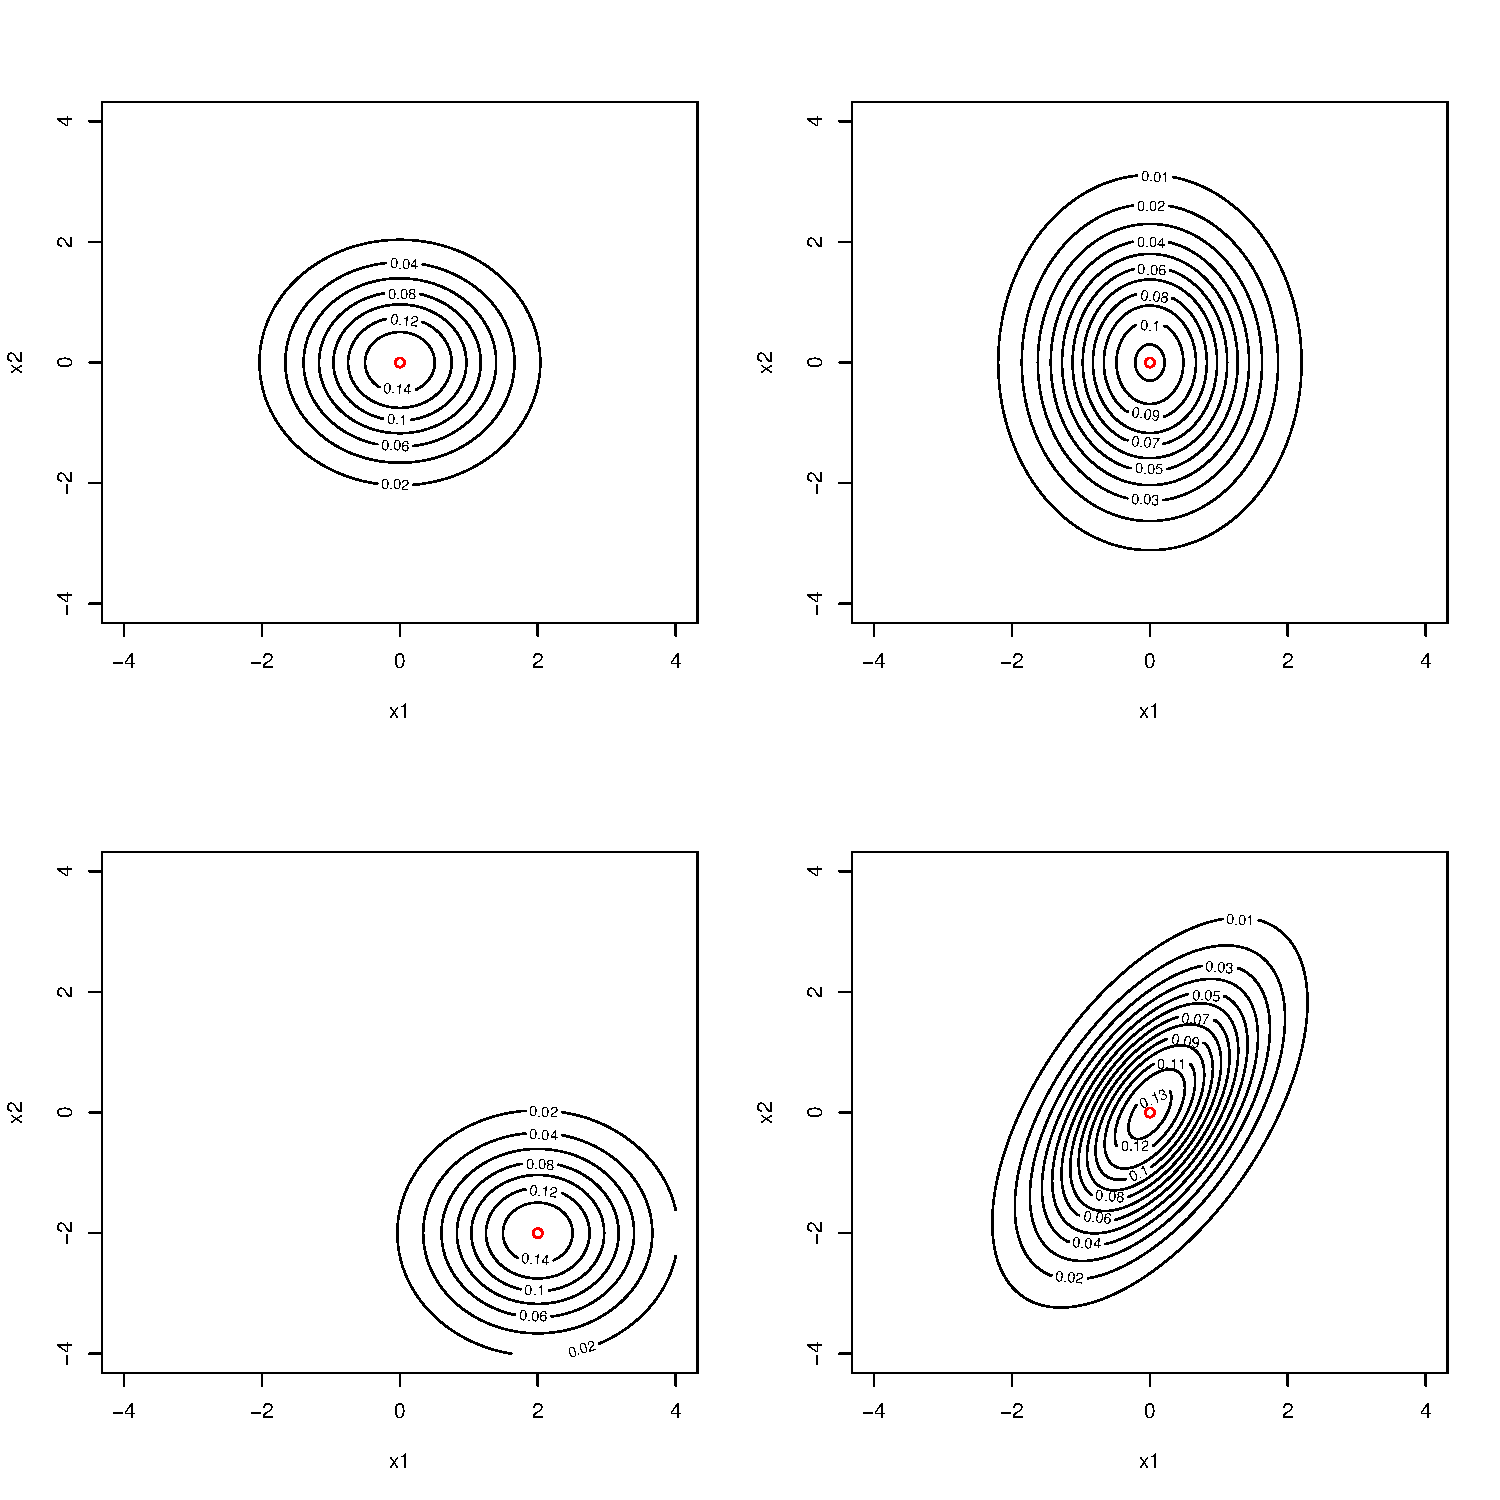
\includegraphics[width=\maxwidth]{figures/multiGauss-1} 

\end{knitrout}
\caption{Multigauss}
\label{fig:multiGauss}
\end{figure}

How is all of this accomplished? By decomposing the covariance matrix, we have already seen that the covariance mostly depends on the eigenvalues of the covariance matrix.
In fact, since scaling is done by $ U\Lambda^{\nicefrac{1}{2}} U^{-1} $, it is the square roots of the eigenvalues that define the spread. They are the dimension-wise 
standard deviations. The matrix of eigenvectors $ U $ transforms any given input into the eigenspace of $ \Sigma $. Since this eigenspace has the same dimensionality
as the original space and $ U $ is normal, $ U $ only performs a rotation.
The matrix $ \Lambda $ performs the same mapping as $ \Sigma $, only in eigenspace. As we have seen, this mapping is much simpler in eigenspace because $ \Lambda $ is
diagonal. If there is no covariance, $ \Sigma = \Lambda $ and thus $ U=I $, meaning no rotation takes place. 
It is only when we introduce covariance that the orientation of the
axis of our coordinate system changes (because transforming a vector in eigenspace is the same as transforming the base vectors of the vector's space into
eigenvectors). The process of computing the multivariate Gaussian density can thus be broken down 
into 3 steps: map into eigenspace, apply the transformation given by $ \Lambda $ and map back into the original space. 

Notice that in Figure~\ref{fig:multiGauss} we only show the plane that the two-dimensional Gaussian is defined on and annotate certain ellipses on that plane with
density values. We give another visualisation in Figure~\ref{fig:3dgauss} where we put the density on top of that plane.

\begin{figure}
\begin{knitrout}
\definecolor{shadecolor}{rgb}{0.969, 0.969, 0.969}\color{fgcolor}
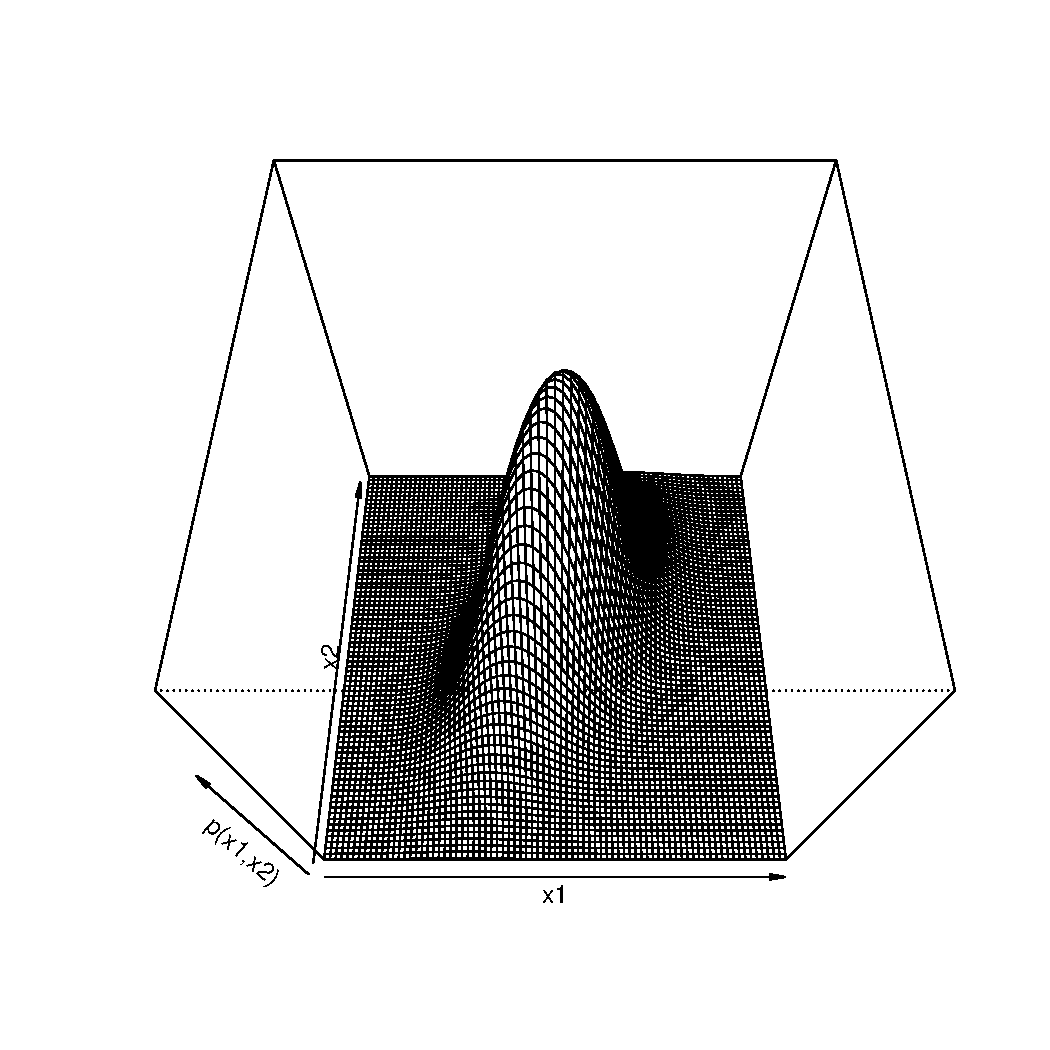
\includegraphics[width=\maxwidth]{figures/3dgauss-1} 

\end{knitrout}
\caption{Gaussian density on top of the 2d plane. The density is the same as the one used in the lower right corner of Figure~\ref{fig:multiGauss}.}
\label{fig:3dgauss}
\end{figure}

\subsection{Marginal and Conditional Distributions}

Now that we have a thorough understanding of the multivariate normal distribution, let us look how to compute its marginal and conditional distributions.

\paragraph{Marginal Distribution} First we re-arrange the dimensions in such a way that the $ k $ dimensions that whose marginal distribution we want to compute
are the first $ k $ dimensions\footnote{This re-arrangement is not necessary but makes the exposition easier.}. This can be done by appropriately swapping the rows and 
columns in the covariance matrix and adjusting the mean vector. Computing the marginal of the first $ k $ dimensions then comes down to projecting the 
$ n $-dimensional RV $ \vec{X} \sim \N{\vec{\mu}}{\Sigma} $ onto its first $ k $ dimensions. To make this explicit, we will represent the mean and covariance matrix
as
\begin{equation}
\vec{\mu} = \begin{bmatrix}
\vec{\mu}_{a} & \vec{\mu}_{b}
\end{bmatrix} \hskip 3cm
\Sigma = \begin{bmatrix}
\Sigma_{aa} & \Sigma_{ab} \\
\Sigma_{ba} & \Sigma_{bb}
\end{bmatrix}
\end{equation}
where part $ a $ contains the $ k $ dimensions we want to project onto and part $ b $ contains the other $ n-k $ dimensions. The appropriate projection matrix
is
\begin{equation}
P = \begin{bmatrix}
I & 0 \\
0 & 0
\end{bmatrix}
\end{equation}
where the identity matrix is of dimension $ k \times k $. It follows that $ PX = Y \sim \N{\vec{\mu_{a}}}{\Sigma_{aa}} $ where $ Y \in \mathbb{R}^{k} $.

\paragraph{Conditional Distribution}

\subsection{Speeding Up Computation}

In this subsection we will look at techniques to make computations with multivariate Gaussians more efficient.

\paragraph{L(ower)U(pper) Decomposition}


\paragraph{Cholesky Decomposition}

\end{document}
